\documentclass{beamer}

\usepackage{amsmath,amsfonts}
\usepackage[T1]{fontenc}
\usepackage[utf8]{inputenc}
%\setmainfont{Droid Serif}

\mode<presentation>
{
%\usetheme{PaloAlto}
%\useoutertheme{tree}
\usecolortheme{lily}
\useinnertheme{rectangles}
\setbeamercovered{transparent}
\setbeamertemplate{blocks}[rounded][shadow=true]
}

\begin{document}

\begin{frame}
  Les slides sont disponibles sur
  \begin{center}
    \centerline{\url{https://github.com/cemosis/unistra.ufr.math}}
  \end{center}
\end{frame}

\section{Analyse Fonctionnelle Avanc{\'e}e et Applications aux EDP}

\begin{frame}\frametitle{Analyse Fonctionnelle Avancée et  EDP}
  \begin{block}{Objectifs}
    \begin{itemize}
    \item Pr{\'e}paration du M2MF 2015-2016
    \item Acquisition du vocabulaire et des outils math{\'e}matiques n{\'e}cessaires {\`a}
      l'analyse des {\'e}quations aux d{\'e}riv{\'e}es partielles
    \end{itemize}
  \end{block}
  \begin{block}{Objets}
    {\'E}tant donn{\'e} $\Omega \subset \mathbb{R}^d, d=1,2,3$, les espaces $H^s(\Omega)$
    \begin{equation*}
      H^s(\Omega)=\{ u \in L^2(\Omega)~,~\forall\alpha \le s,~D^\alpha u\in L^2(\Omega)\}
    \end{equation*}
  \end{block}
  \begin{block}{Questions}
    \begin{itemize}
    \item Propri{\'e}t{\'e}s de ces espaces
    \item Applications aux EDP: cadre fonctionel pour montrer
      l'existence et unicit{\'e} de solutions
    \end{itemize}
  \end{block}
\end{frame}

\begin{frame}\frametitle{Analyse Fonctionnelle Avancée et EDP}

  \begin{block}{Quelques exemples d'EDP: probl\`emes d'\'evolution}

Evolution d'une solution en temps $t$ sur un domaine $\Omega$. La solution est donn\'ee implicitement par une \'equation, des conditions limites (au bord du domaine)
et une donn\'ee initiale. Formalisation sous la forme
$$
\frac{d u}{dt}+Au = 0,\ u(0) = u_0
$$

{\bf Equation de la chaleur:} mod\'elise la distribution de temp\'erature $u$ dans un domaine $\Omega$ \`a l'instant $t$

$$
\partial_t u -\Delta u = 0
$$

{\bf Equation des ondes:} mod\'elise %les petites vibrations d'une corde (en dimension $1$) ou d'une membrane \'elastique (en dimension $2$), ou plus g\'en\'eralement
la propagation d'une onde (acoustique, \'electromagn\'etique...)

$$
\partial_t^2u-\Delta u = 0
$$

R\'ef\'erence: Ha\"im Brezis, Analyse Fonctionnelle

  \end{block}


\end{frame}


\section{Méthodes Numériques pour les EDP}

\begin{frame}{M{\'e}thodes Num{\'e}riques pour les EDP}


  \begin{columns}
    \column{.5\linewidth}
    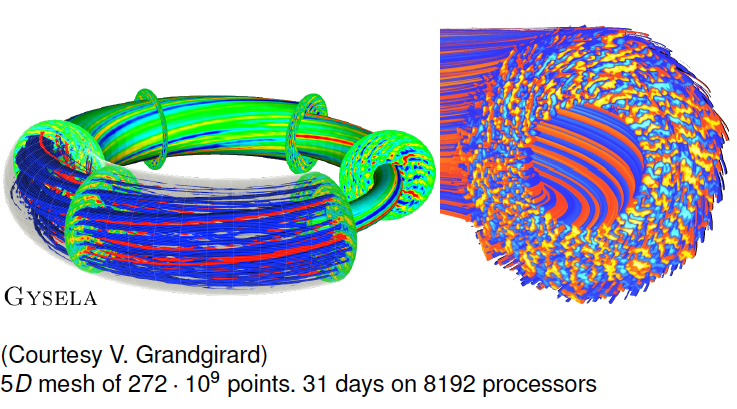
\includegraphics[width=0.9\linewidth]{gysela.png}\\
    \centerline{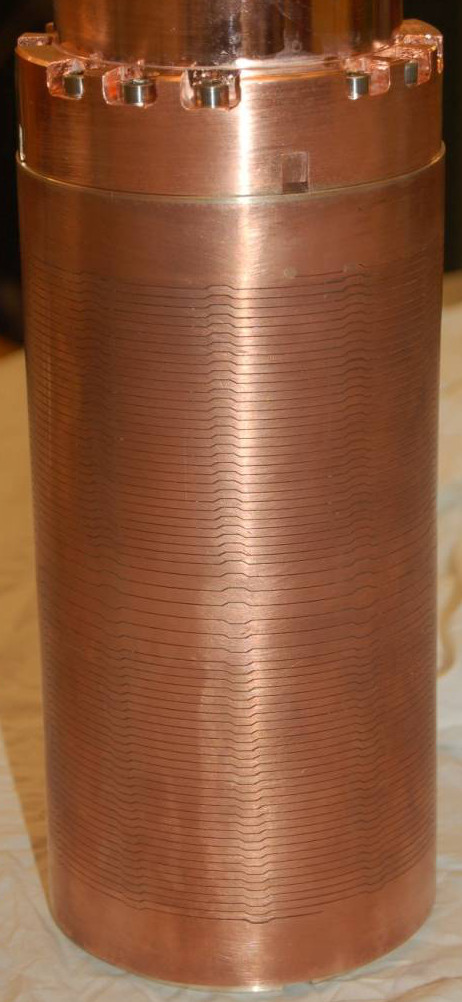
\includegraphics[height=4cm]{Radial_magnet.jpg}\quad
    \includegraphics[height=4cm]{temperature.jpg}}
    \column{.5\linewidth}
    \centerline{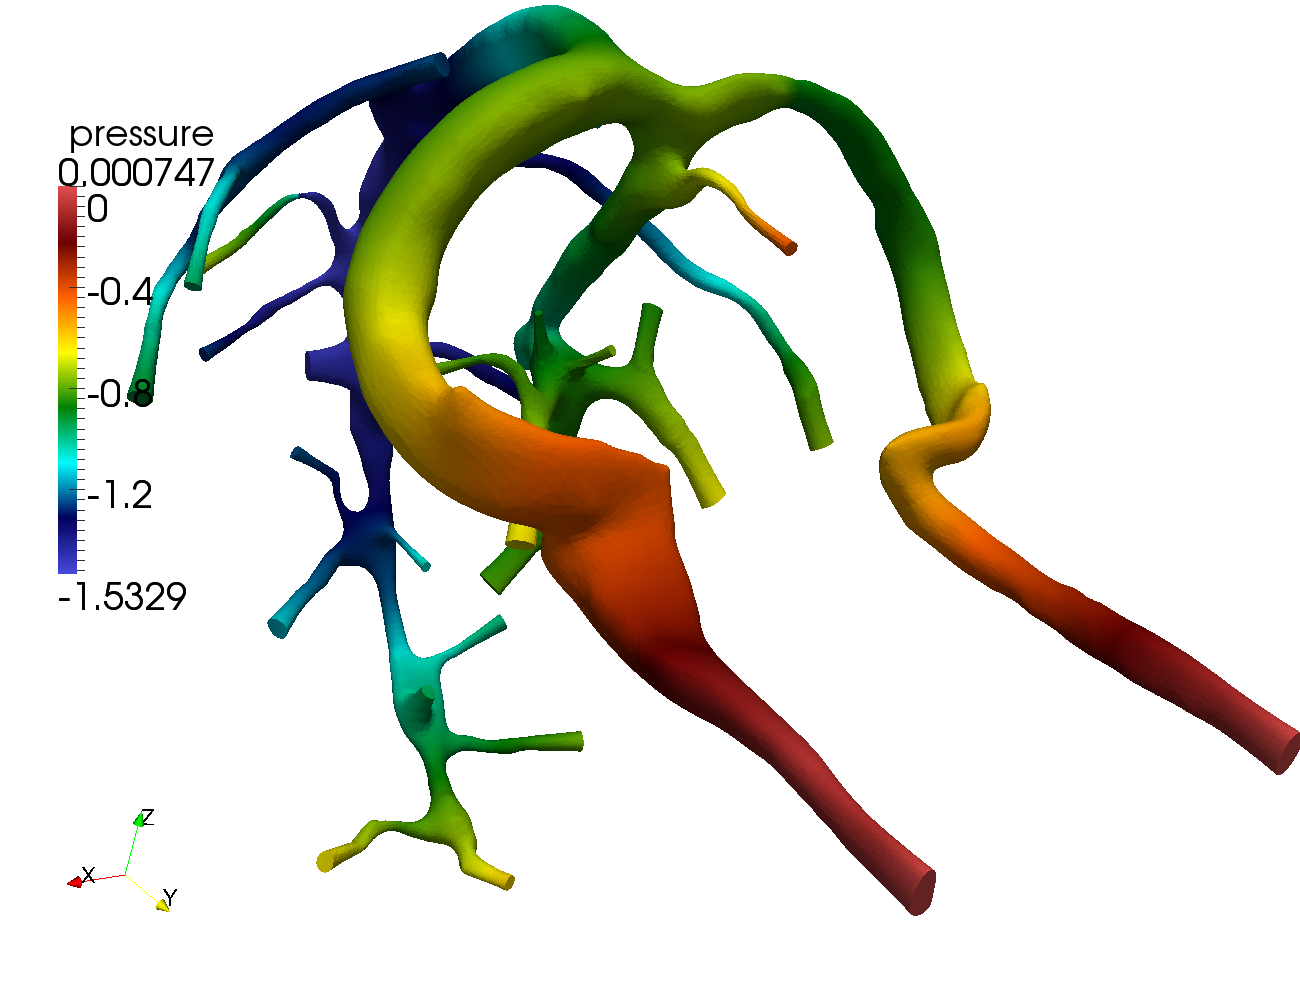
\includegraphics[width=.9\linewidth]{MesoChallengePressure.png}}\\
    \centerline{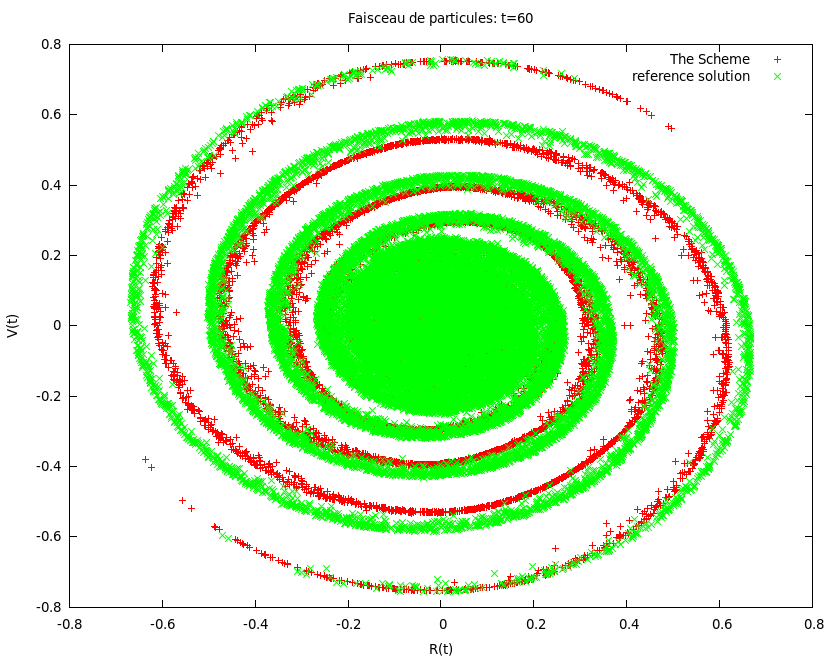
\includegraphics[width=.9\linewidth]{hirstoaga.png}}
  \end{columns}




\end{frame}
\begin{frame}{Méthodes Numériques pour les EDP: Rao \& Prud'homme}
  \begin{block}{Objectifs}
    \begin{itemize}
    \item {\'E}tude math{\'e}matique et num{\'e}rique de la m{\'e}thode des {\'e}l{\'e}ments
      finis qui propose un cadre g{\'e}n{\'e}ral pour passer de formulations
      continues {\`a} discr{\`e}tes
    \item le cadre th{\'e}orique est donn{\'e} par le cours d'Analyse
      Fonctionnelle Avanc{\'e}e
    \end{itemize}
  \end{block}
  \begin{block}{Questions}
    \begin{itemize}
    \item Existence et unicit{\'e} de solution pour des probl{\`e}mes
      elliptiques lin{\'e}aires coercifs aux niveaux continu et discret
    \item Construction de fonctions de bases, dites {\'e}l{\'e}ment fini
    \item Erreur d'interpolation et d'approximation en norme $L^2$ et $H^1$
    \item Impl{\'e}mentation de la m{\'e}thode et V{\'e}rification num{\'e}riques des th{\'e}or{\`e}mes
    \end{itemize}
  \end{block}
\end{frame}

\begin{frame}{Vers le M2}

  \begin{block}{M2R EDP 2015-2016}
    Dans le cadre du M2, les cours couvrent les aspects théoriques et
    approximations numériques.
    \begin{itemize}
    \item Systèmes hyperboliques (B. Rao, P. Helluy)
    \item Réductions de modèles
      \begin{itemize}
      \item Méthodes des bases réduites (C. Prud'homme)
      \item Méthodes multi-échelles pour des équations de transport (S. Hirstoaga)
      \end{itemize}
    \item EDP paraboliques
      \begin{itemize}
      \item Théorie et approximation (Z. Belhachmi)
      \item Application à l'interaction
        fluide-structure (C. Murea)
      \end{itemize}
    \end{itemize}
  \end{block}

\end{frame}
\end{document}
